%!TEX program = xelatex
\documentclass[xcolor={table}]{beamer}

\usepackage[brazil]{babel}	
\usepackage[utf8]{inputenc}
\usepackage[T1]{fontenc}
\usepackage[scaled]{helvet}
\usepackage{amsthm}
\usepackage{ragged2e}
\usepackage{subfig}
\usepackage[table]{xcolor}
\usepackage{multicol}
\usepackage{multirow}
\usepackage{fancyvrb}
\usepackage{verbatim}
\usepackage{wrapfig}
\usepackage{lipsum}  
\usepackage{listings}
\usepackage{url}
\usepackage{graphicx}
\usepackage{hyperref}
\usepackage{tikz}
\def\checkmark{\tikz\fill[scale=0.6](0,.35) -- (.25,0) -- (1,.7) -- (.25,.15) -- cycle;} 

\usepackage{geometry}
\geometry{rmargin=0.2in,bmargin=0.2in}


\usetheme{Execushares}

   \begin{subfigure}
           \hspace*{0.1in}

        \vspace*{0.2in}
           
\includegraphics[scale=0.45]{img/URJC_logo.png}
            \label{fig:urjc}
        \end{subfigure}
        \begin{subfigure}
            
\includegraphics[scale=0.36]{img/betsitLogo.png}
            \label{fig:etsit}
        \end{subfigure}

\vspace{0.8cm}
\title{Mejoras en entorno de robótica  educativa para niños}
\subtitle{Trabajo de fin de grado}
\author{Rubén Álvarez Martín}
\date{19 de Diciembre, 2019}

\begin{document}
	\setcounter{showProgressBar}{0}
	\setcounter{showSlideNumbers}{0}

	\frame{\titlepage}

	\begin{frame}
		\frametitle{Índice}
		\begin{enumerate}
			\item Introducción  \textcolor{ExecusharesGrey}{}
		 \textcolor{ExecusharesGrey}{\footnotesize\hspace{0.5em}}
 		\item Objetivos  \textcolor{ExecusharesGrey}{}
		 \textcolor{ExecusharesGrey}{\footnotesize\hspace{0.5em}}
			\item Herramientas  \textcolor{ExecusharesGrey}{\footnotesize\hspace{0.5em}}
			\item Mejoras a WebSim  \textcolor{ExecusharesGrey}{
			\begin{itemize}
			    \item Soporte a drones en WebSim
			    \item Teleoperadores en WebSim
			    \item Ejercicios individuales
			    \item Ejercicios competitivos
			\end{itemize}} 
			\item Conclusiones  \textcolor{ExecusharesGrey}{\footnotesize\hspace{0.5em}}
		\end{enumerate}
	\end{frame}

	\setcounter{framenumber}{0}
	\setcounter{showProgressBar}{1}
	\setcounter{showSlideNumbers}{1}
	\section{Introducción}
		\begin{frame}

			\frametitle{Tecnologías web}
			\begin{itemize}
			    \begin{itemize}
    			    \item HTTP
    			    \item Tecnologías cliente: HTML5, CSS3 y JS. 
    			    \item Tecnologías servidor: Node, Django y Spring. 
			    \end{itemize}{}
			\end{itemize}
			
		\begin{figure}[H]
        \centering
        \begin{subfigure}{\textwidth}
            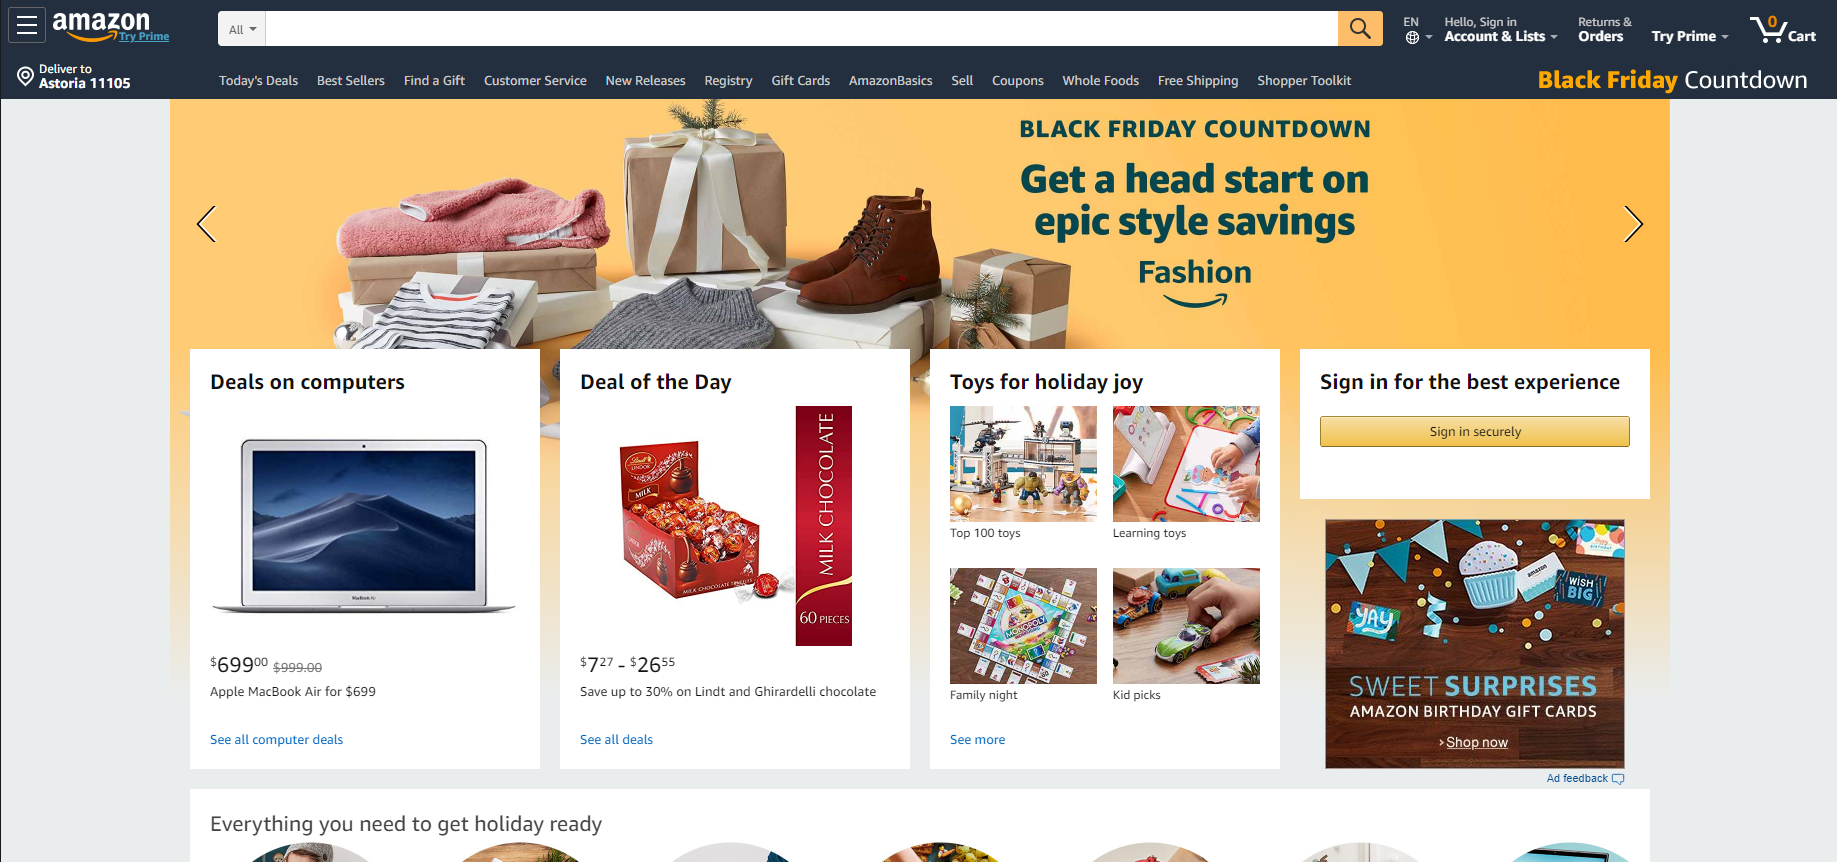
\includegraphics[width=5.5cm, height=4cm]{img/amazon.png}
        \label{fig:amazon}
        \end{subfigure}\hfill
        \begin{subfigure}{\textwidth}
            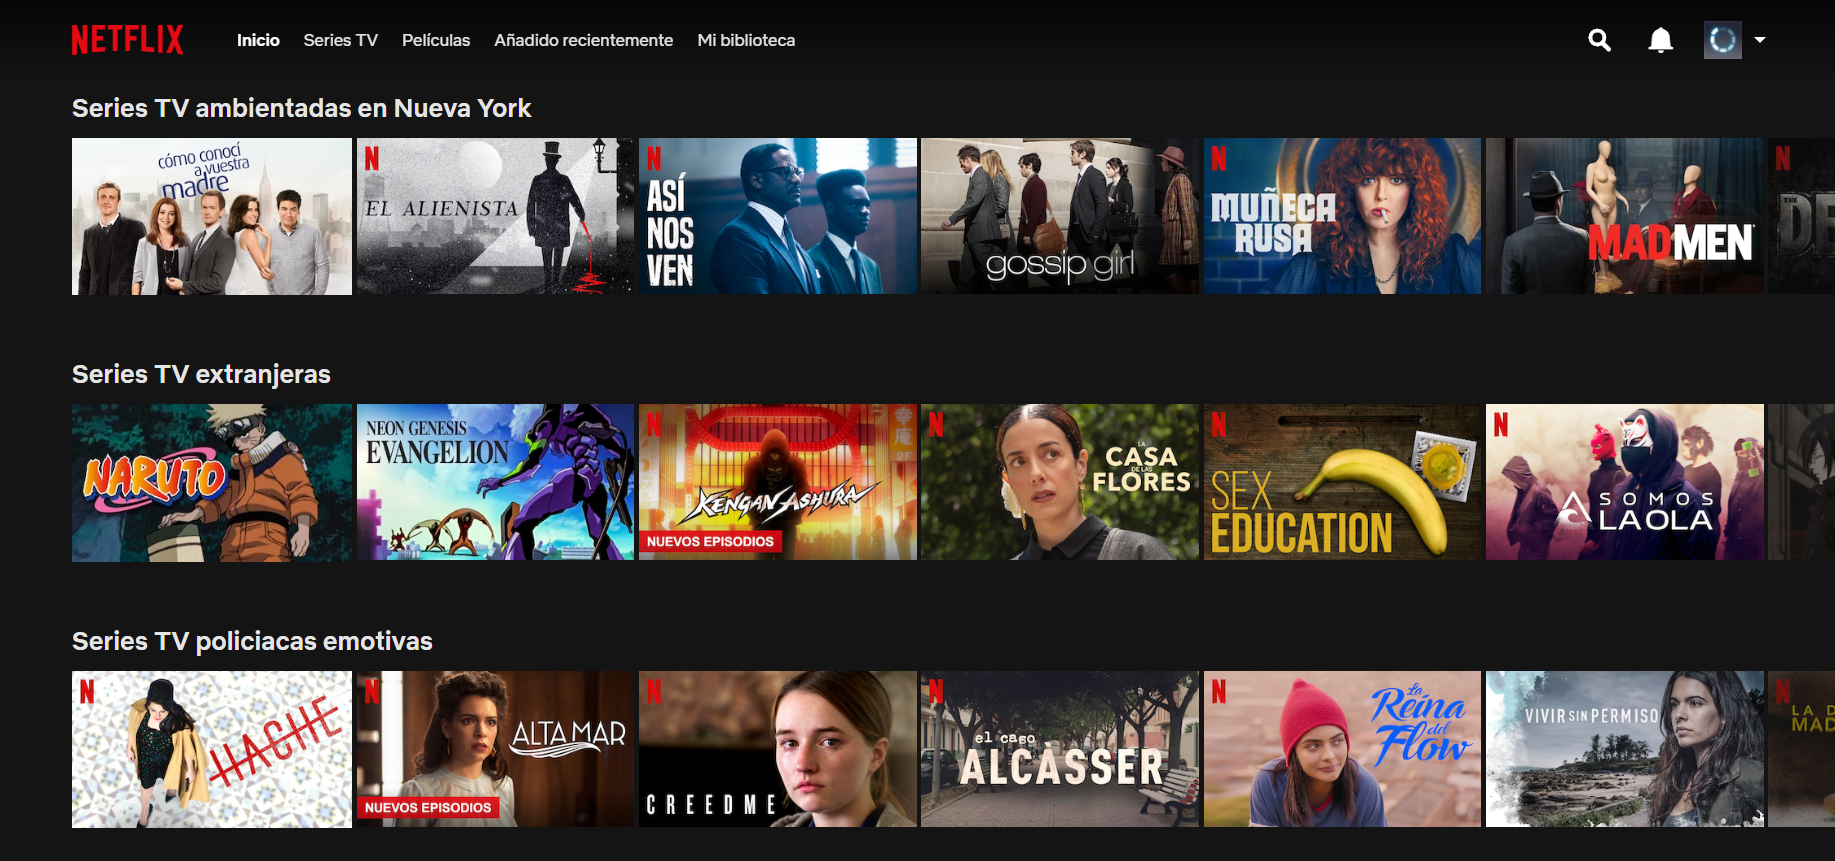
\includegraphics[width=5.5cm, height=4cm]{img/netflix.png}
        \label{fig:netflix}
        \end{subfigure}\hfill
            \label{fig:appwebs}
            \end{figure}
		\end{frame}
		
		
		\begin{frame}
		\frametitle{Robótica}
        \begin{figure}[H]
        \centering
        \begin{subfigure}{\textwidth}
            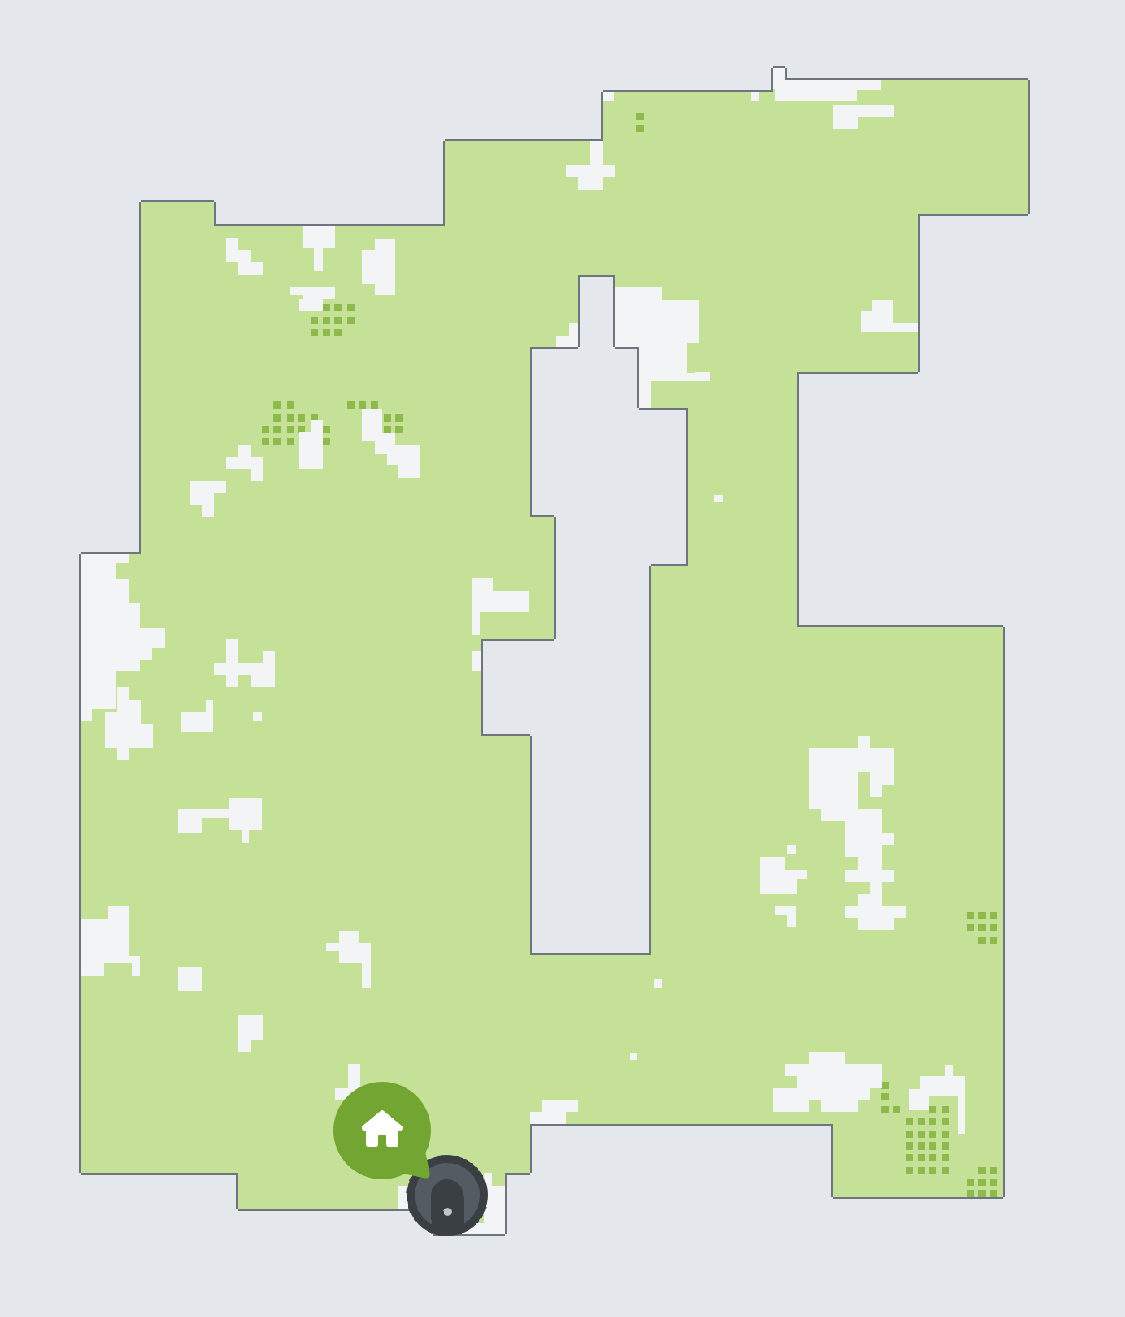
\includegraphics[width=3cm, height=3cm]{img/roomba.png}
        \label{fig:roomba}
        \end{subfigure}\hfill
        \begin{subfigure}{\textwidth}
            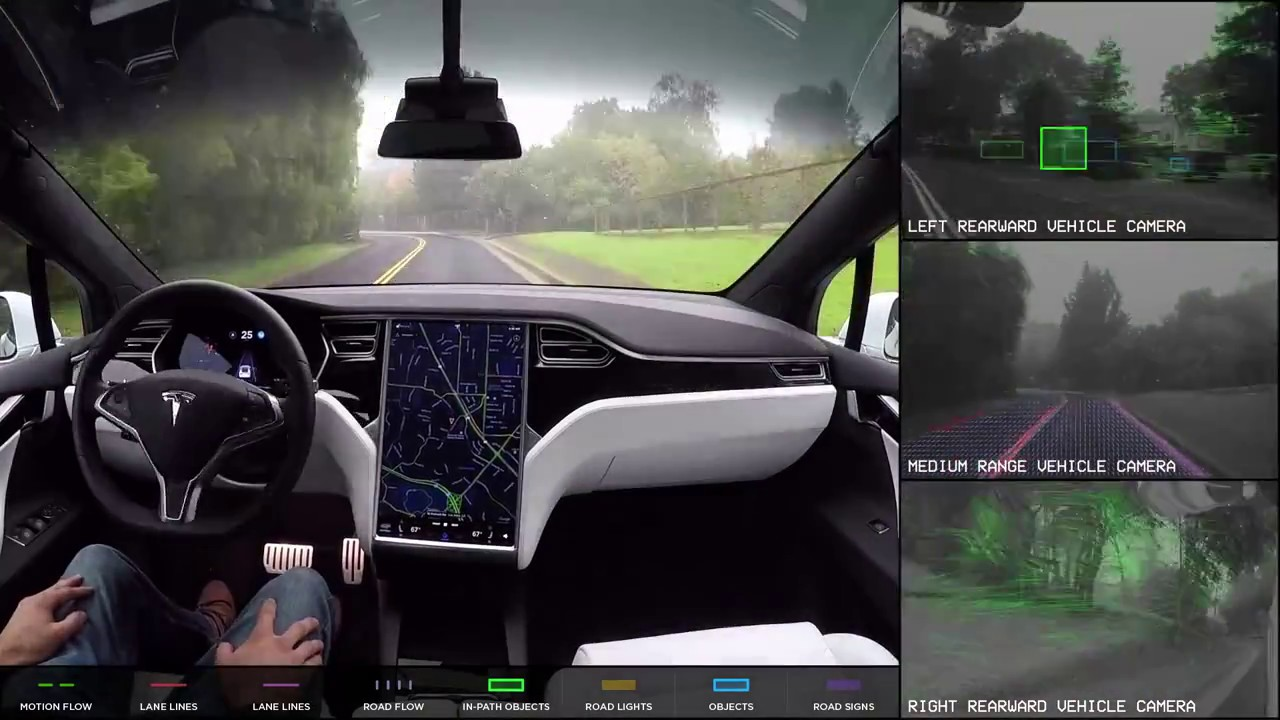
\includegraphics[width=6cm, height=3.5cm]{img/tesla.jpg}
        \label{fig:tesla}
        \end{subfigure}\hfill
        \label{fig:robotica}
        \end{figure}
            \begin{itemize}
                \begin{itemize}
                    \item \textit{robot} = \textit{hardware} + \textit{software}
                    \item \textit{hardware} = sensores + actuadores + procesadores
                \end{itemize}            \end{itemize}{}
		\end{frame}
		
	\begin{frame}
		\frametitle{Robótica educativa}
		\begin{itemize}
	          \item Plataformas hardware: \textit{LEGO mindstorm}, \textit{mBot} o \textit{Arduino}.
        \begin{figure}[H]
        \centering
        \begin{subfigure}{\textwidth}
            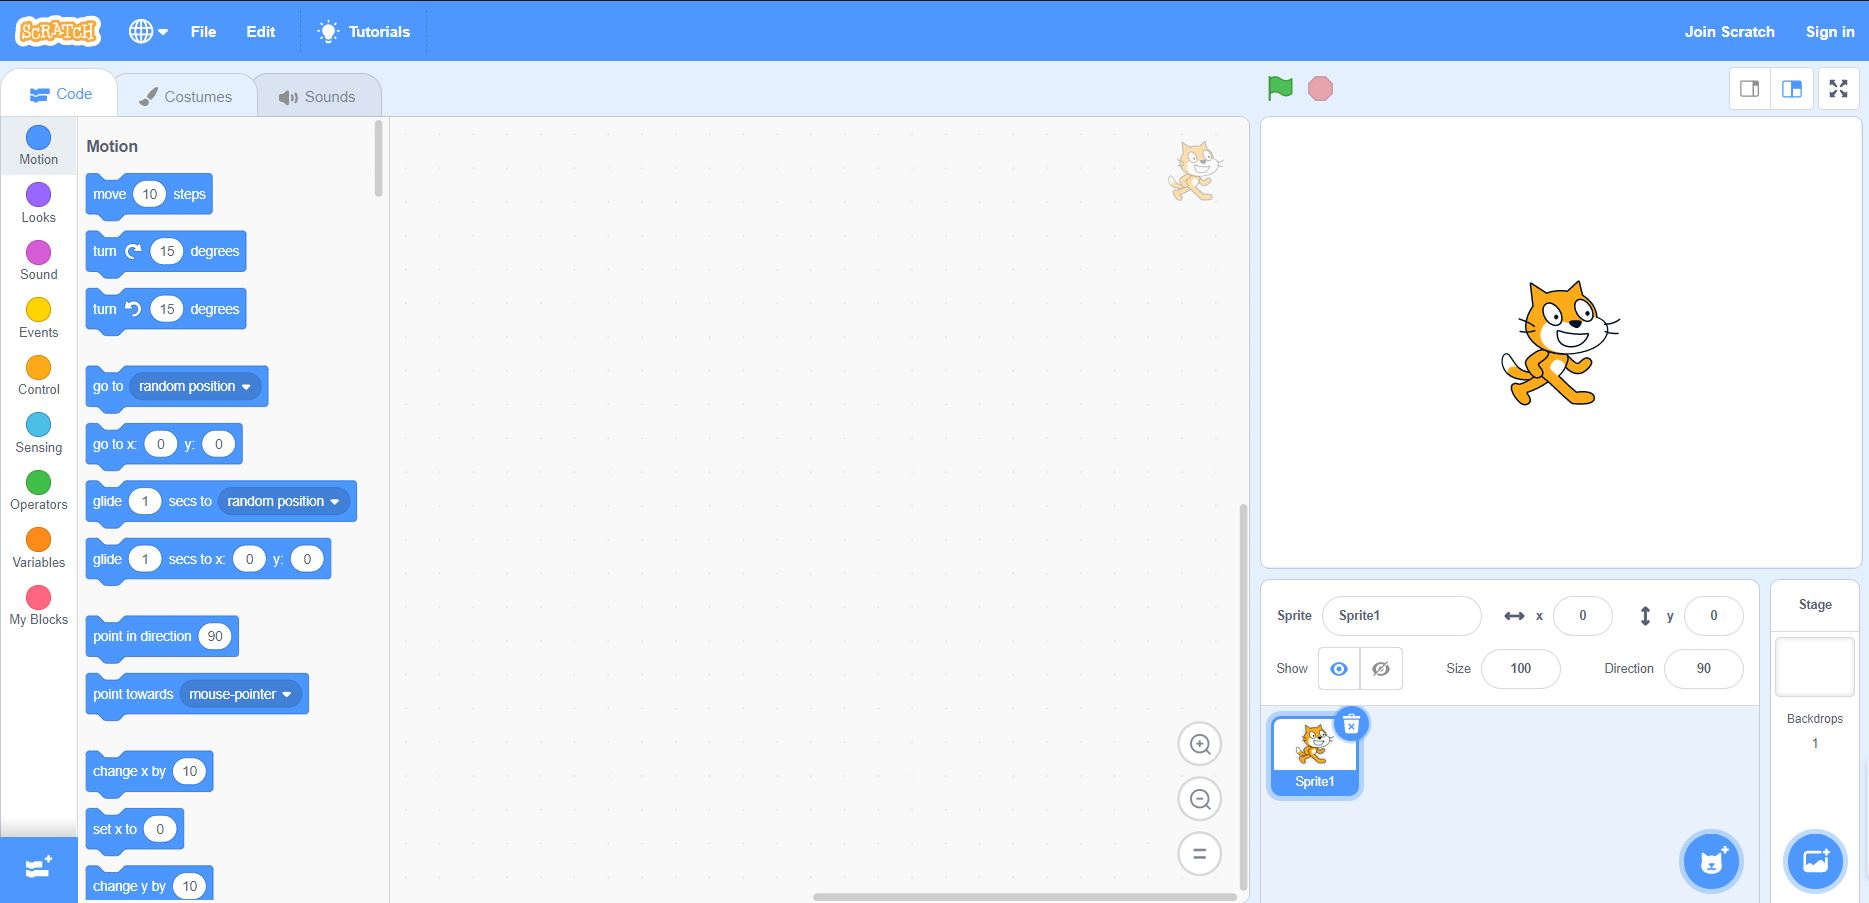
\includegraphics[scale=0.13]{img/scratch.jpg}
        \label{fig:scratch}
        \end{subfigure}\hfill
        \begin{subfigure}{\textwidth}
            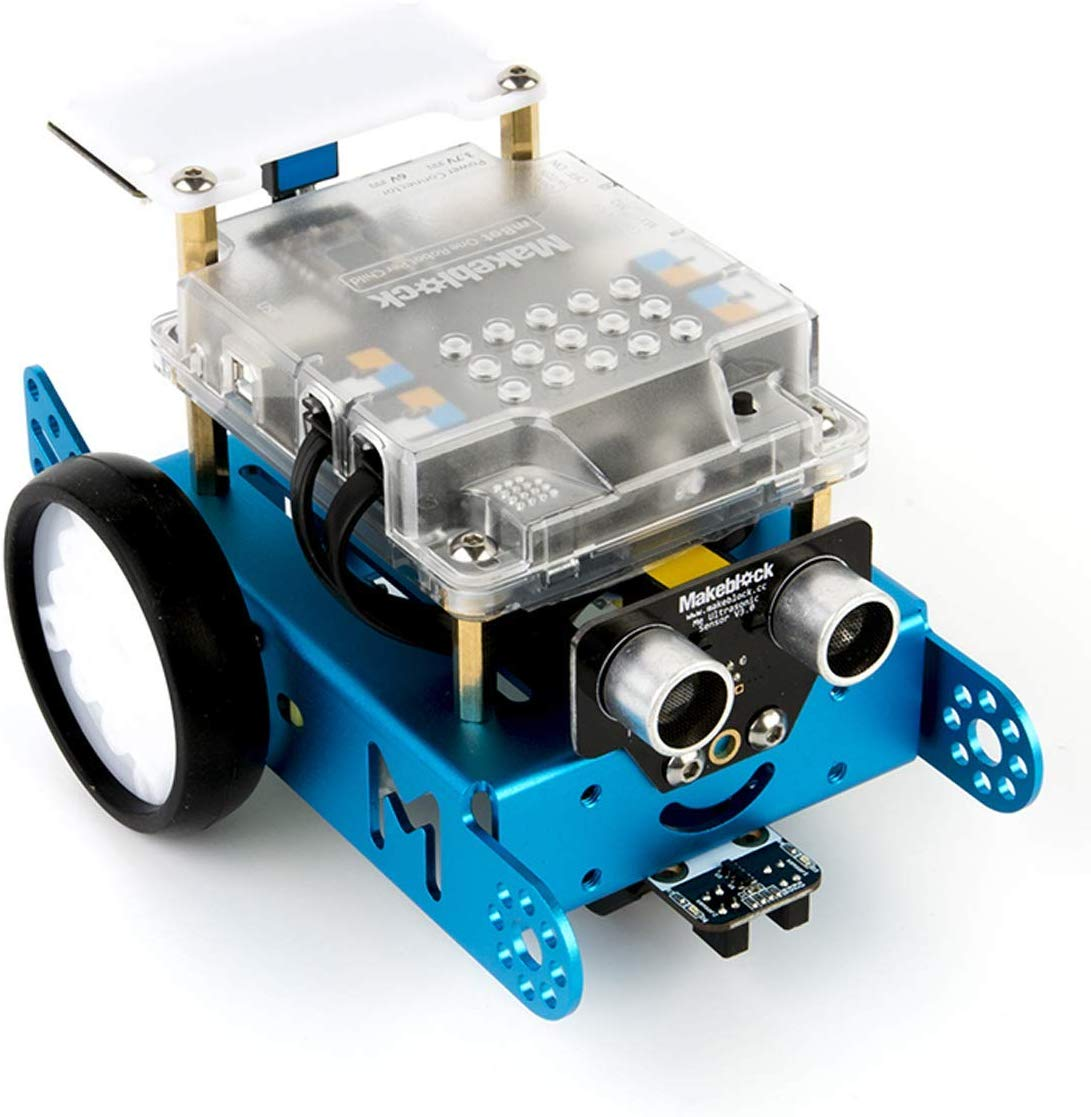
\includegraphics[scale=0.1]{img/mBotReal.jpg}
        \label{fig:mbot}
        \end{subfigure}\hfill
            \label{fig:educativa}
        \end{figure}
        	\item Lenguajes de programación visual: Scratch, Snap! o Kodu.
  
		\end{itemize}
	\end{frame}

	\section{Objetivos}
		\begin{frame}
			\frametitle{Objetivos}
			\begin{itemize}\itemsep4pt
			    \item Mejorar \textit{WebSim}:
			    \begin{enumerate}\itemsep5pt
			        	\item Soporte a \textit{drones}.
				\item Teleoperadores y ficheros de configuración.
				\item Ejercicios individuales. 
				\item Ejercicios competitivos y evaluadores automáticos. 
			    \end{enumerate}{}
			
			\end{itemize}
		\end{frame}

	\section{Herramientas}
		\begin{frame}
			\frametitle{Herramientas}
                \begin{figure}[H]
                \centering
                \begin{subfigure}{\textwidth}
                    
\includegraphics[width=3cm, height=3cm]{img/js.png}
                \label{fig:figure2_4}
                \end{subfigure}
                \begin{subfigure}{\textwidth}
                    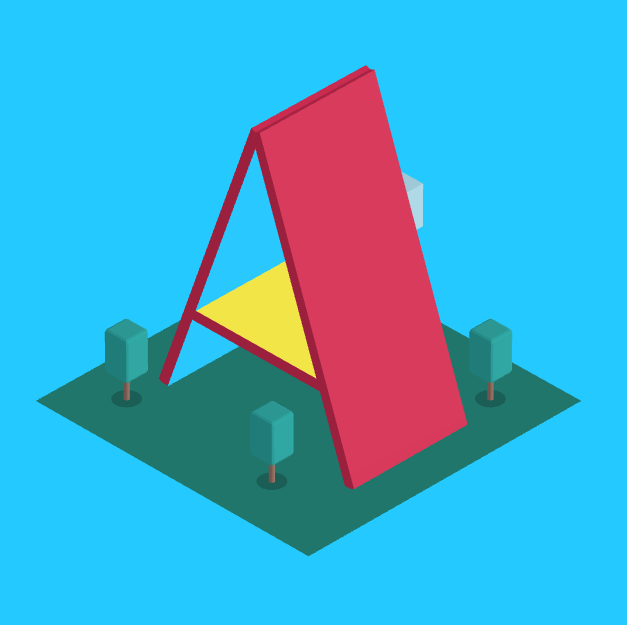
\includegraphics[width=3cm, height=3cm]{img/aframe.png}
                \label{fig:figure2_5}
                \end{subfigure}\hfill
                \begin{subfigure}{\textwidth}
                    
\includegraphics[width=3cm, height=3cm]{img/blockly.png}
                \label{fig:figure2_6}
                \end{subfigure}\hfill
                \begin{subfigure}{\textwidth}                    
\includegraphics[width=3cm, height=3cm]{img/blender.png}
                \label{fig:figure2_7}
                \end{subfigure}\hfill
                \begin{subfigure}{\textwidth}                      
\includegraphics[width=3cm, height=3cm]{img/webpack.jpeg}
                    \label{fig:figure2_9}
                    \end{subfigure}\hfill
                    \begin{subfigure}{\textwidth}
                        
\includegraphics[width=3cm, height=2cm]{img/npm.png}
                    \label{fig:figure2_8}
                    \end{subfigure}\hfill
                    \label{fig:herramientas}
                    \end{figure}
        \end{frame}
        
        
	\begin{frame}
	\frametitle{WebSim}
	    \begin{figure}
	        \centering
	        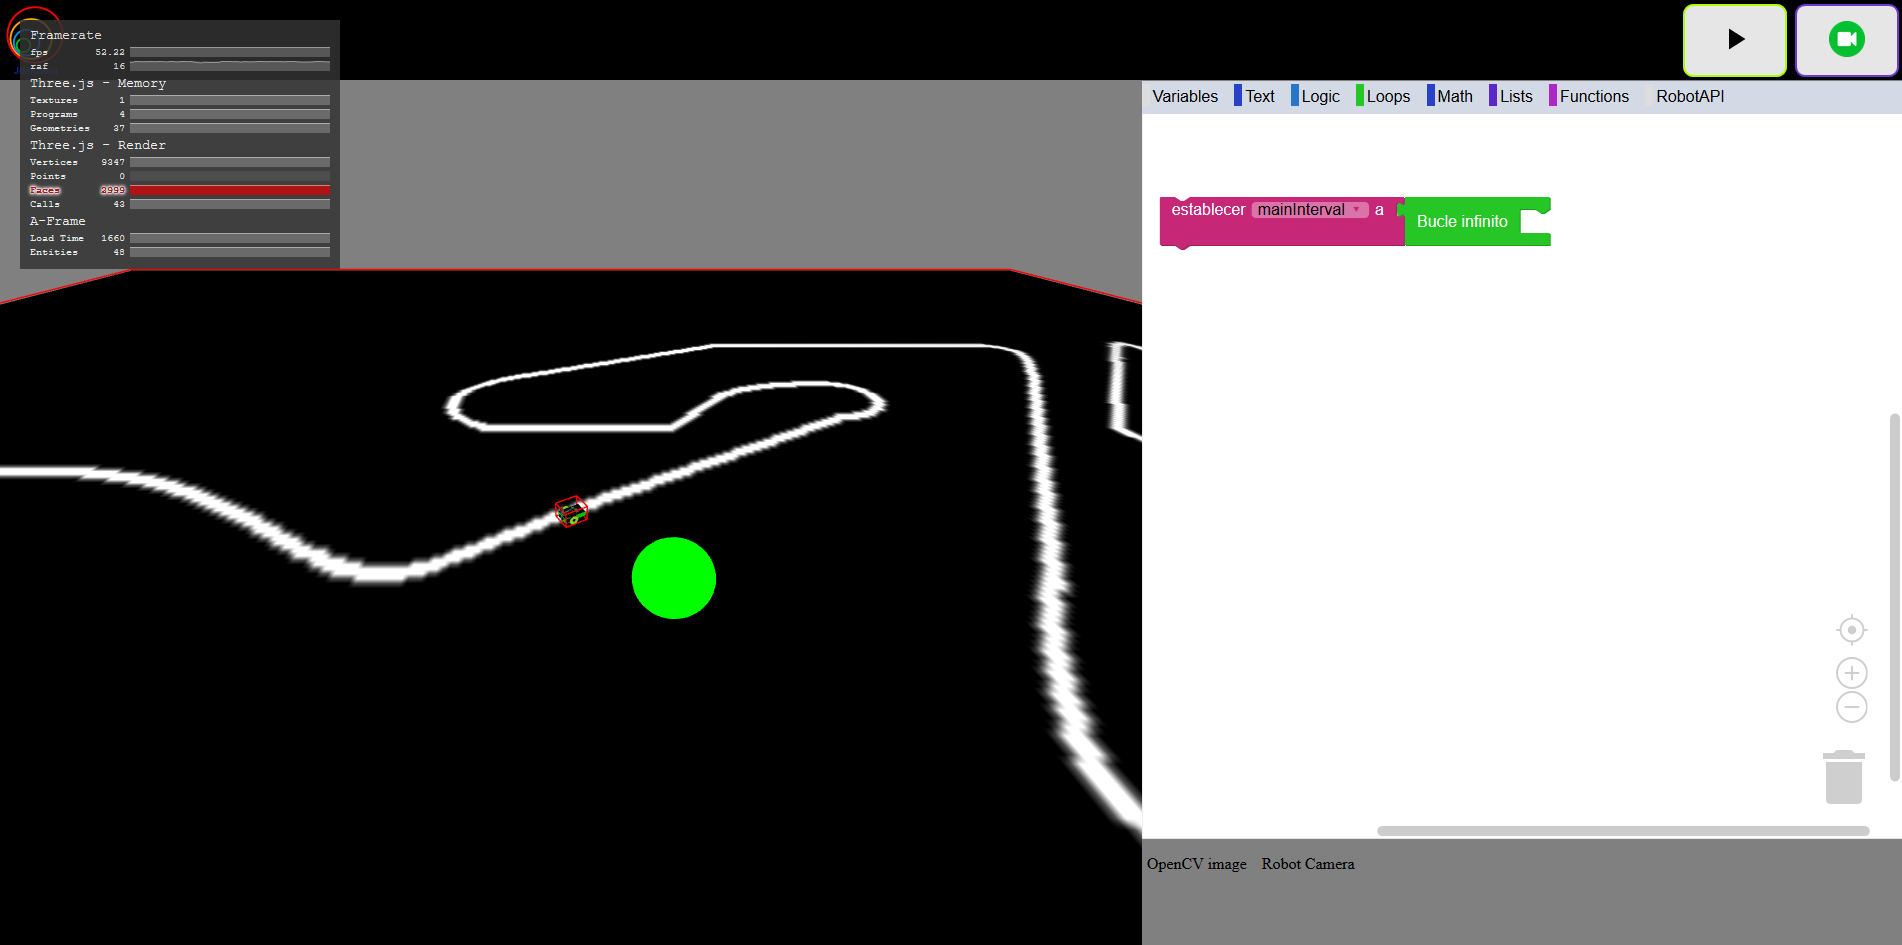
\includegraphics[width=0.85\textwidth]{img/interfaz-websim.png}
	        \label{fig:websim}
	    \end{figure}
	    \begin{itemize}
            \begin{itemize}
    	    \item \textit{WebSim} -> simulador web robótico  para enseñar conceptos básicos de tecnología, robótica y programación (Álvaro Paniagua).
	     \end{itemize}{}
	\end{itemize}
\end{frame}
		
	\section{Mejoras a WebSim}


    	\begin{frame}
			\frametitle{Soporte a drones: Modelo 3D}
      \begin{minipage}{.48\textwidth}
      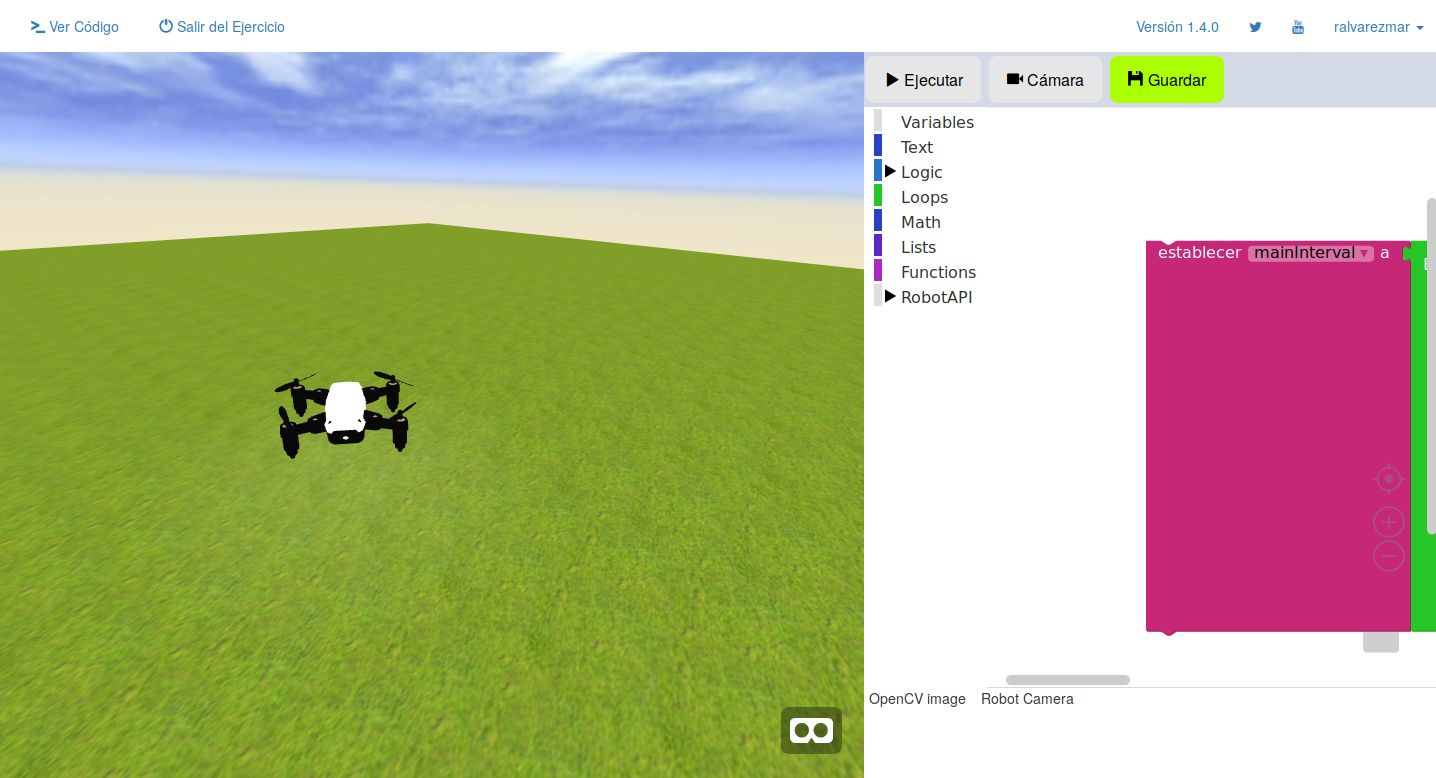
\includegraphics[scale=0.25]{img/WebsimDrone.png}
        \end{minipage}
      \begin{minipage}{.50\textwidth}
      \begin{itemize}
      \begin{itemize}{}\itemsep5pt
          \item Formato \textit{A-Frame}
          \item Modelo \textit{low-poly}
          \item Animación hélices
          \end{itemize}
      \end{itemize}
    \end{minipage}
    	\end{frame}

		\begin{frame}
		\frametitle{Soporte a drones: Drivers}
		\begin{itemize}
		    \begin{itemize}
		    \item \textbf{HAL API}: Sensores y actuadores.
		    \end{itemize}
		\end{itemize}
\begin{table}[H]
  \begin{center}
    \vspace{0.5cm}
    \label{tab:tablaMotores2}
    \begin{tabular}{|c|c|} 
    \hline
      \textbf{Método} & \textbf{Descripción}\\
      \hline
.setL(integer) & \begin{tabular}[c]{@{}c@{}}Comanda velocidad ascendente\\\end{tabular} \\ \hline
.getL() & \begin{tabular}[c]{@{}c@{}}Devuelve velocidad ascendente\\\end{tabular} \\ \hline
.despegar() & \begin{tabular}[c]{@{}c@{}}Despega \textit{drone}\\ \end{tabular} \\ \hline
.aterrizar() & \begin{tabular}[c]{@{}c@{}}Aterriza \textit{drone} \\ \end{tabular} \\ \hline
.move(integer, integer, integer) & \begin{tabular}[c]{@{}c@{}}Comanda velocidades\\ \end{tabular} \\ \hline
  \textit{setVelocity()} & \begin{tabular}[c]{@{}c@{}}Materializa velocidad y posición \\ \end{tabular} \\ \hline
    \end{tabular}
  \end{center}
\end{table}
\end{frame}


		\begin{frame}
		\frametitle{Soporte a drones: Bloques Scratch}
		 \begin{minipage}{.45\textwidth}
		       \begin{figure}[H]
            \centering
            
\includegraphics[scale=0.5]{img/ascensionBlockly.png}
           \label{fig:ascension}
            \end{figure}
                 \begin{figure}[H]
            \centering
            
\includegraphics[scale=0.4]{img/verticalBlockly.png}
           \label{fig:vertical}
            \end{figure}
            \begin{figure}[H]
            \centering
            
\includegraphics[scale=0.48]{img/aterrizarBlockly.png}
           \label{fig:vertica}
            \end{figure}
               \begin{figure}[H]
            \centering
            
\includegraphics[scale=0.5]{img/despegarBlockly.png}
           \label{fig:vertica}
            \end{figure}
                        \end{minipage}
            \begin{minipage}{.48\textwidth}
            \begin{figure}
                \centering                   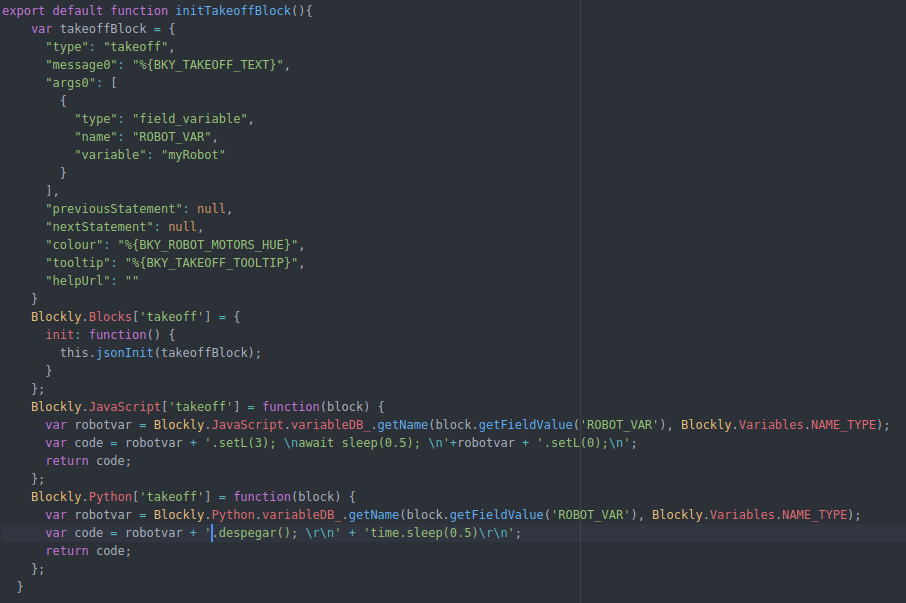
\includegraphics[width=6.2cm, height=5.8cm]{img/traduccionDespegar.png}
                \label{fig:traduccion}
            \end{figure}
            \end{minipage}
		\end{frame}
		
		\begin{frame}
			\frametitle{Otros modelos}
		\begin{figure}[H]
        \centering
        \begin{subfigure}{\textwidth}
         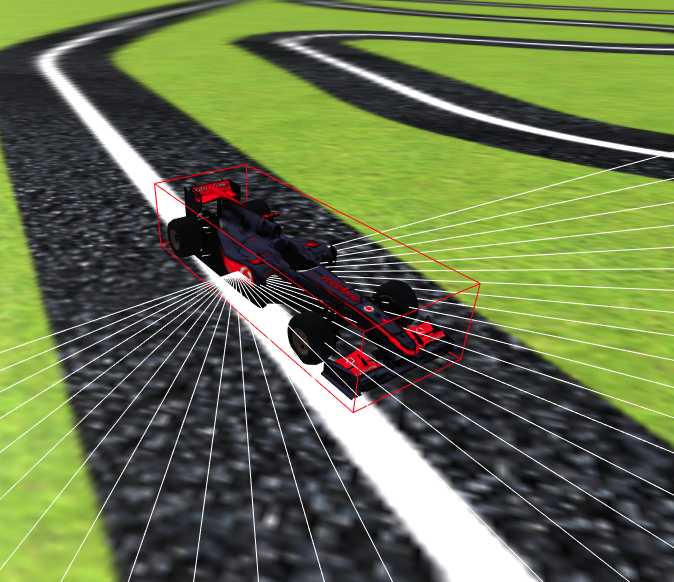
\includegraphics[width=4cm, height=3cm]{img/f1_williams.png}
 \label{fig:f1williams}
        \end{subfigure}
        \begin{subfigure}{\textwidth}
         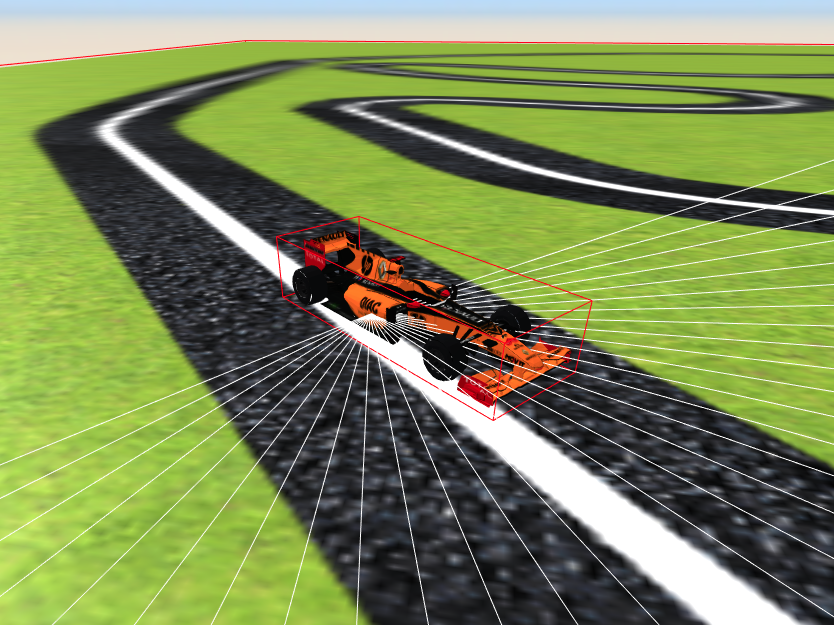
\includegraphics[width=4cm, height=3cm]{img/f1_renault.png}
   \label{fig:f1renault}
        \end{subfigure}
        \begin{subfigure}{\textwidth}
         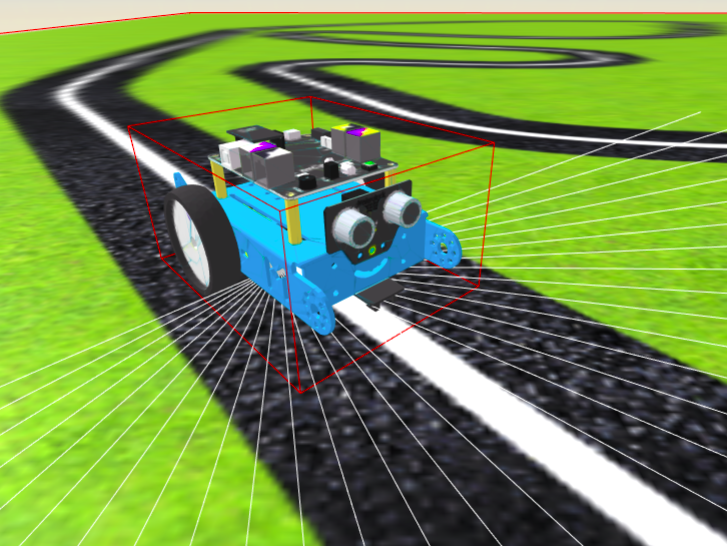
\includegraphics[width=4cm, height=3cm]{img/mBot_model.png}
   \label{fig:mbot}
        \end{subfigure}
        \end{figure}
		\end{frame}
		
		\begin{frame}
		\frametitle{Teleoperadores}
    		\begin{figure}{\textwidth}
    		\centering
             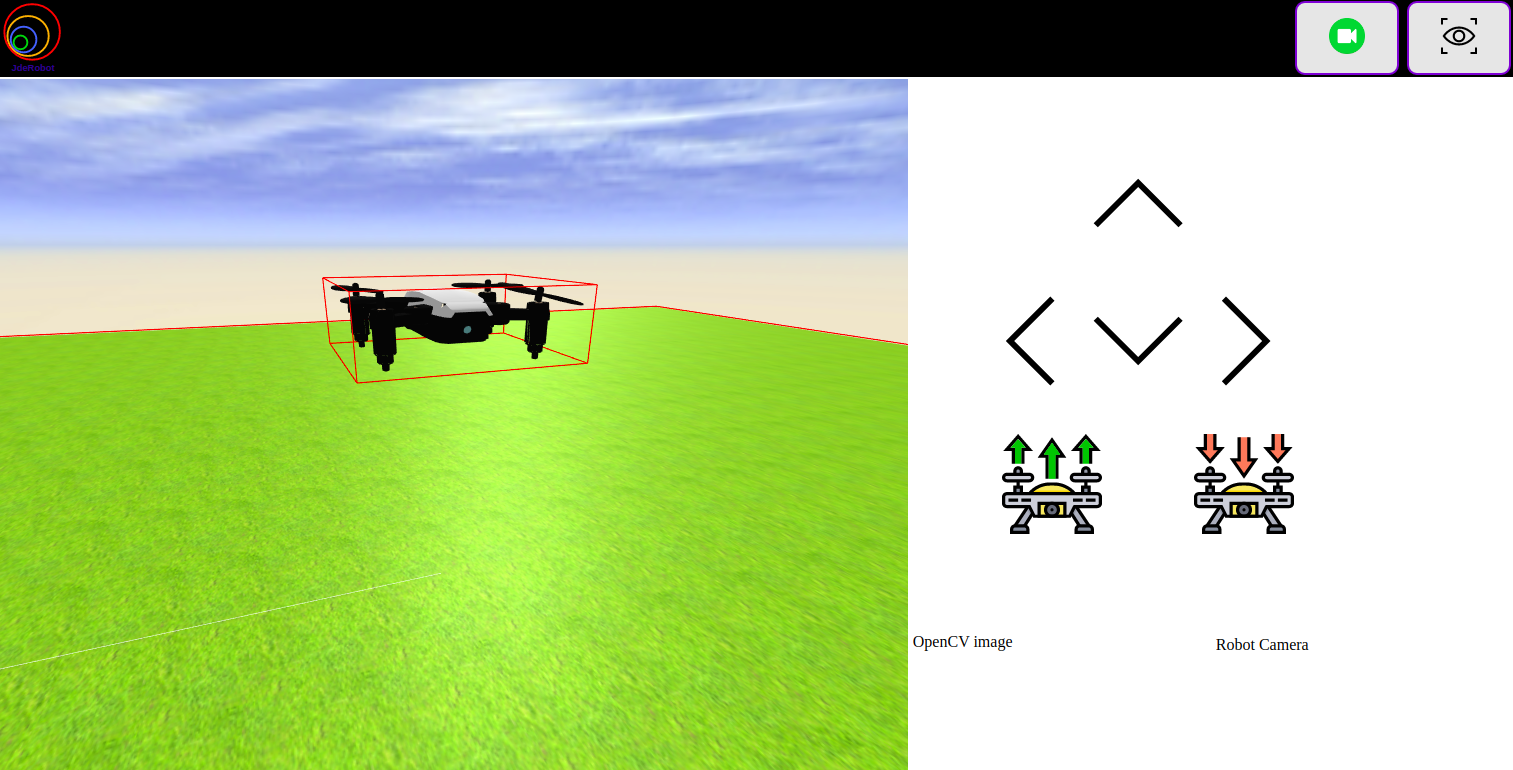
\includegraphics[scale=0.18]{img/drone_teleoperator.png}
             \label{fig:teleopdrone}
            \end{figure}
            	\begin{itemize}
            	\begin{itemize}
    		    	\item Permiten controlar robots sin programarlos.
            	\end{itemize}
		    \end{itemize}
		\end{frame}
		
		\begin{frame}
			\frametitle{Teleoperadores: configuración}
			\newline
		    \begin{itemize}
		        \item Ficheros de configuración ->  crear escenario sin tener elementos en el código fuente.
		        \item Formato JSON ->  escenario,  robot, gravedad, elementos, etc. 
		    \end{itemize}
		\end{frame}
		
		\begin{frame}
			\frametitle{Ejercicios individuales}
	  \begin{figure}[ht]
        \centering
          \begin{subfigure}{\textwidth}
            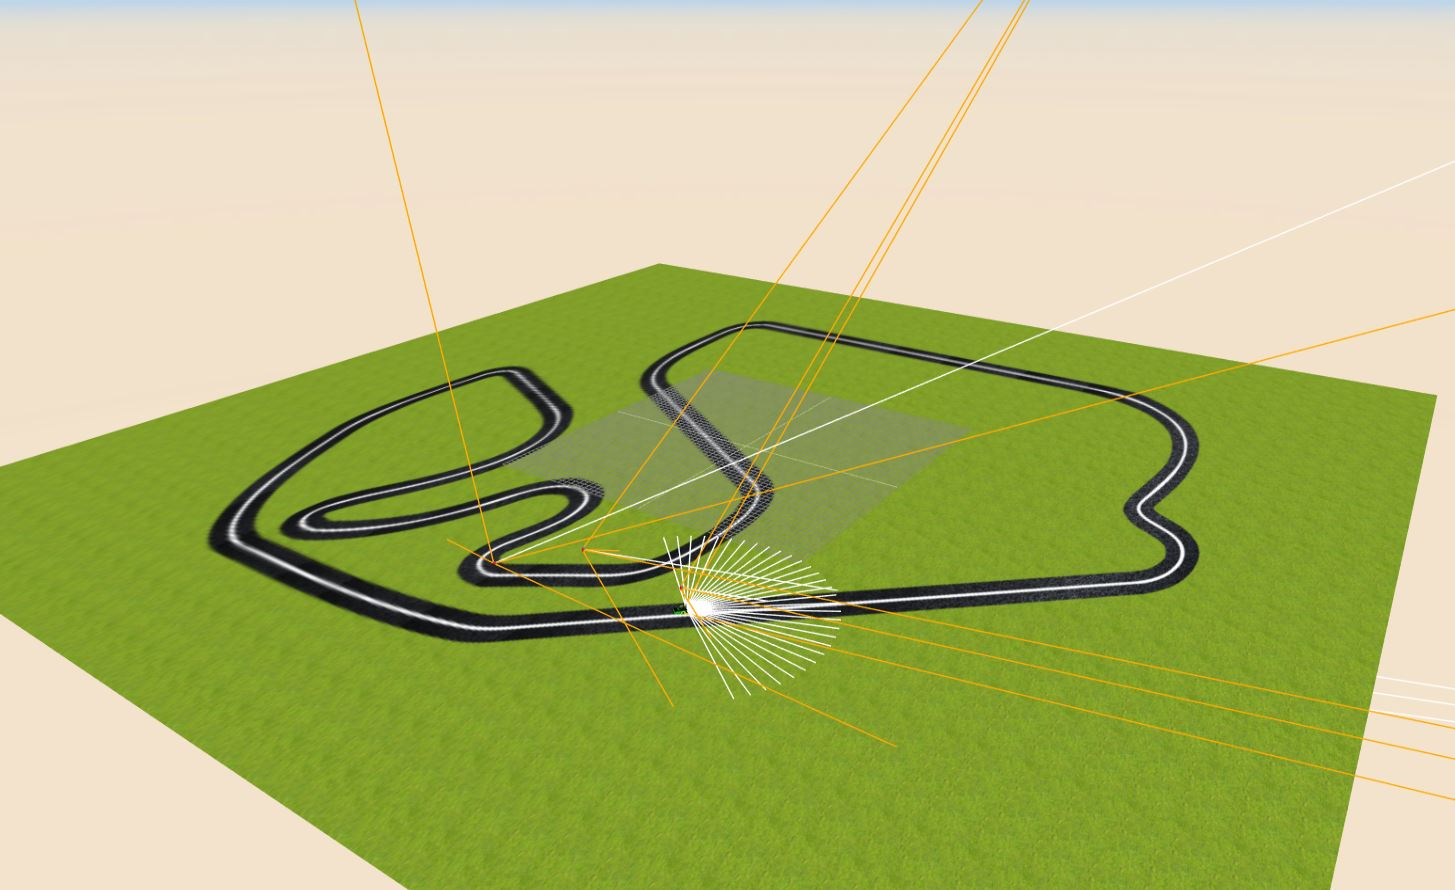
\includegraphics[width=5.5cm, height=3cm]{img/pibot_vision.JPG}
        \label{fig:vision}
        \end{subfigure}\hfill
        \begin{subfigure}{\textwidth}
            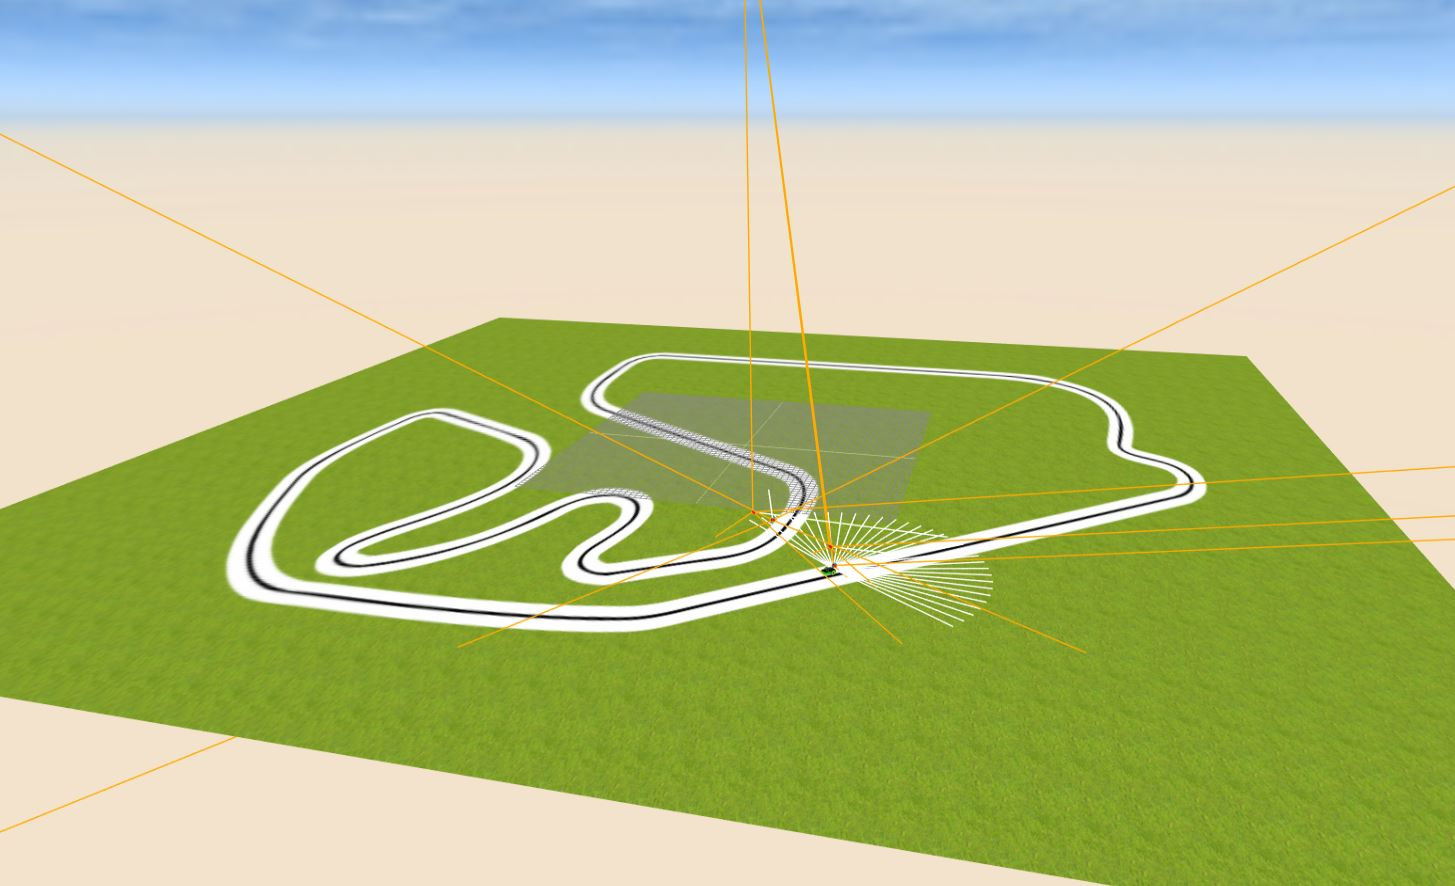
\includegraphics[width=5.5cm, height=3cm]{img/siguelineas_ir.JPG}
        \label{fig:ir}
        \end{subfigure}\hfill
        \begin{subfigure}{\textwidth}
            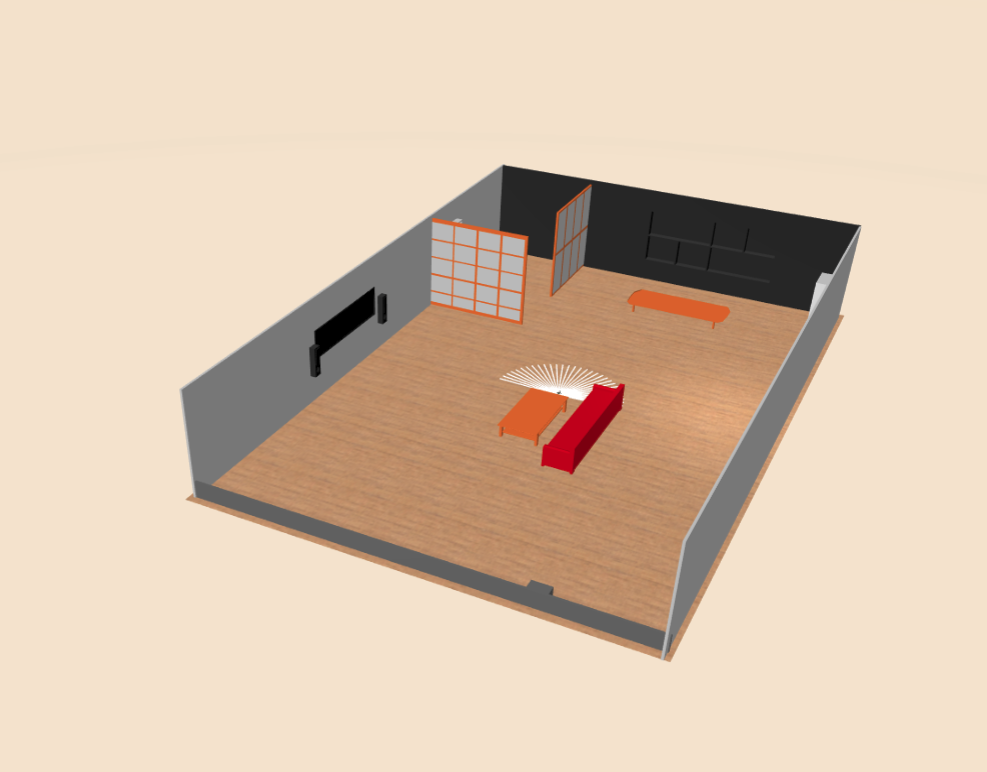
\includegraphics[width=5.5cm, height=3cm]{img/bump&go.png}
        \label{fig:chocagira}
        \end{subfigure}\hfill
        \begin{subfigure}{\textwidth}
            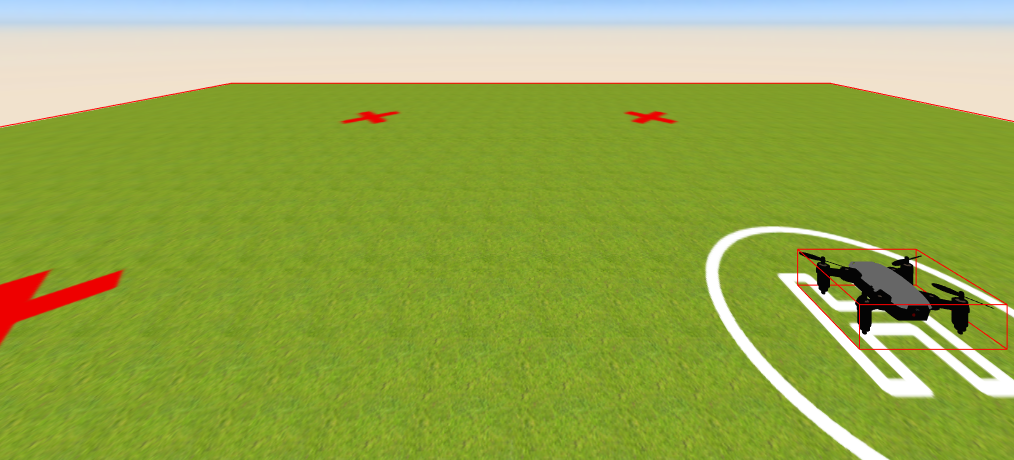
\includegraphics[width=5.5cm, height=3cm]{img/cuadradoDrone.png}
        \label{fig:cuadrado}
        \end{subfigure}
            \label{fig:ejercicios}
            \end{figure}
         \end{frame}
		

		\begin{frame}
			\frametitle{Ejercicios individuales: Sigue pelota}
        \begin{figure}[H]
        \centering
        \begin{subfigure}{\textwidth}
            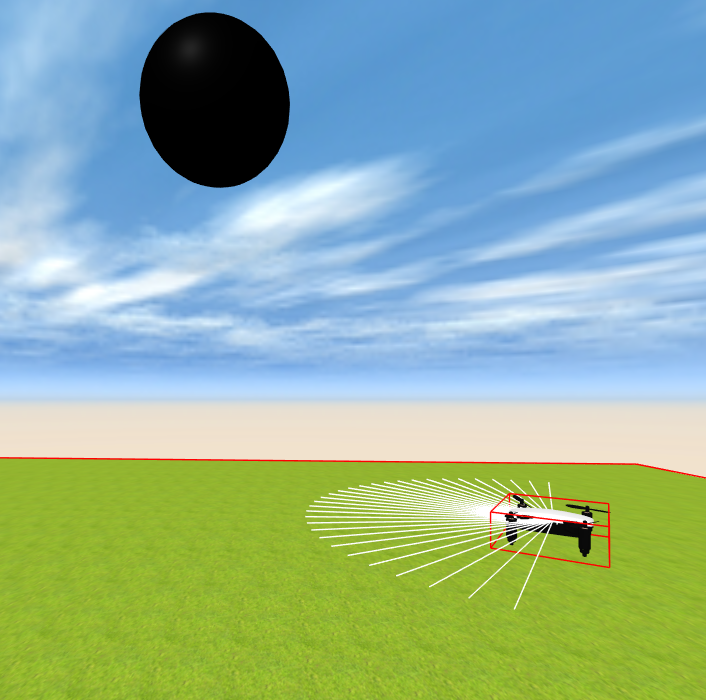
\includegraphics[width=6cm, height=4cm]{img/followBallTello12.png}
        \label{fig:followBall}
        \end{subfigure}\hfill
        \begin{subfigure}{\textwidth}
            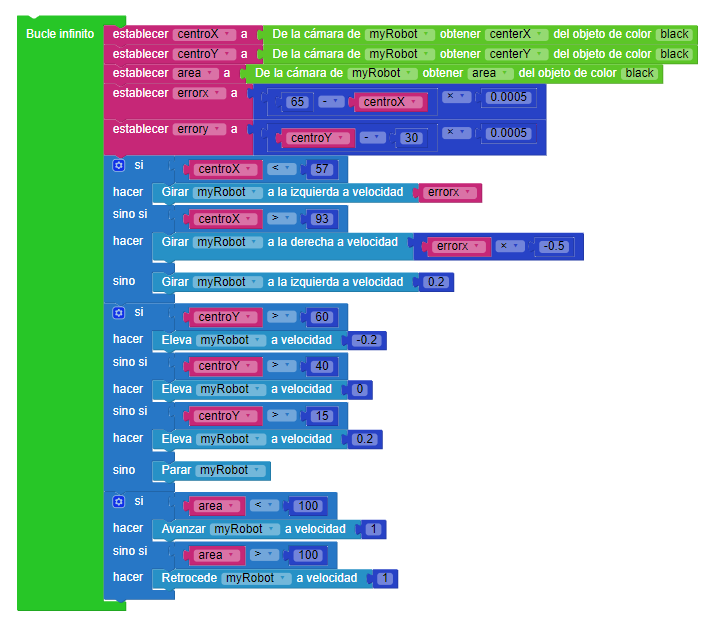
\includegraphics[width=5cm, height=5.5cm]{img/siguepelotacodigo.png}
        \label{fig:siguepelotacodigo}
        \end{subfigure}\hfill
        \label{fig:siguepelota}
        \end{figure}
 		\end{frame}
	
		\begin{frame}
			\frametitle{\LARGE{Ejercicios individuales: Atraviesa bosque}}
       \begin{figure}
       \begin{subfigure}{\textwidth}
         \href{https://youtu.be/z3n47wWHDFc}
              {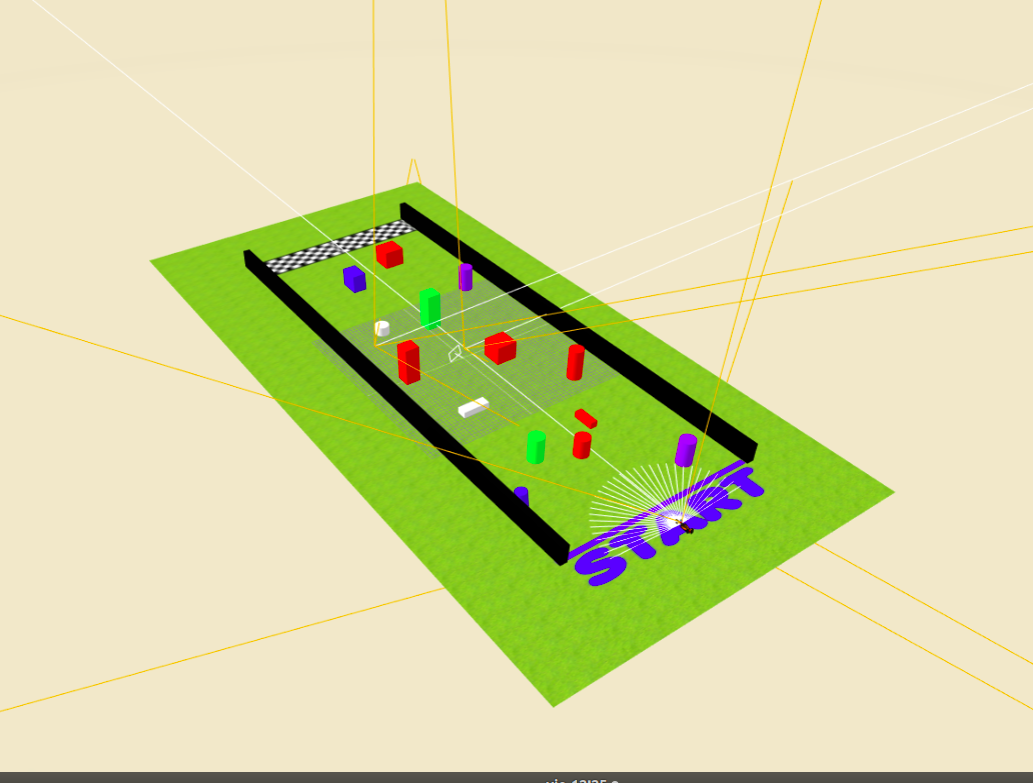
\includegraphics[width=6cm, height=4cm]{img/atraviesabosque-indiv.png}}
       \end{subfigure}
       \begin{subfigure}      
       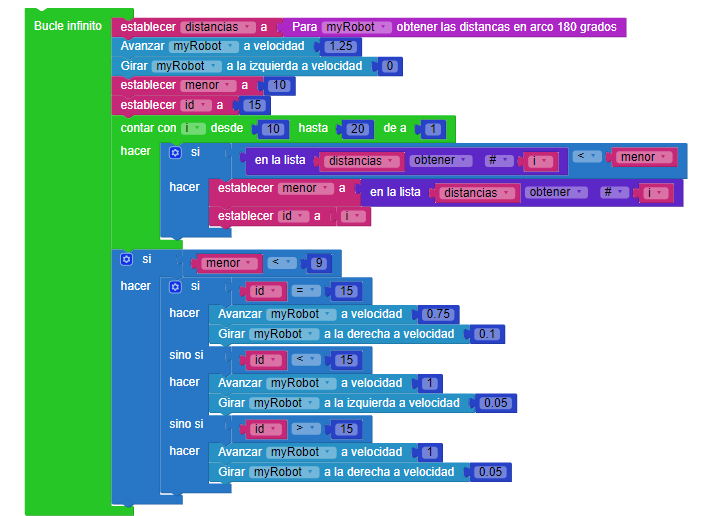
\includegraphics[width=4.5cm, height=5cm]{img/atraviesaBosqueCodigo.png}
       \end{subfigure}
       \end{figure}
       \scriptsize{\url{https://youtu.be/z3n47wWHDFc}}
		\end{frame}
		
		\begin{frame}
			\frametitle{\LARGE{Ejercicios competitivos: Arquitectura}}
			\begin{itemize}
			    \item \large{Módulo \textit{\textbf{brains}} ampliado.}
			    \item \large{Módulo \textit{\textbf{evaluators}}:} \normalsize{\textit{runEvaluator(arrayRobots,evaluator)}}
	
			    \item \large{Módulo \textit{\textbf{agents}}:} \normalsize{\textit{runAgent(idRobot, path)} }
			   
			\end{itemize}
			\begin{figure}
			    \centering			    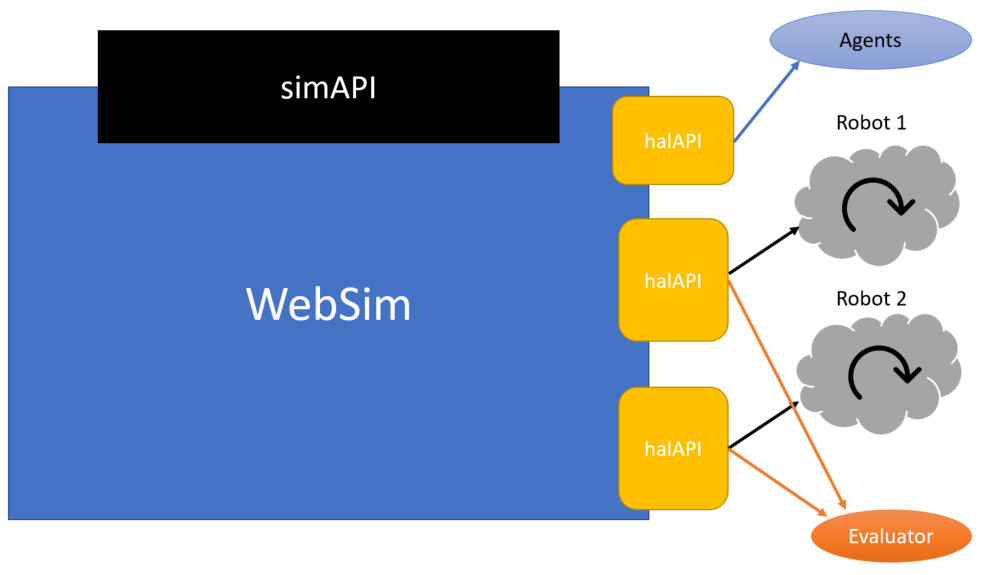
\includegraphics[scale=0.25]{img/arquitectura.png}
			\end{figure}
		\end{frame}
		
		\begin{frame}
			\frametitle{Ejercicios competitivos: Editores}
			\begin{itemize}
			     \item Editores dobles:
			\end{itemize}
				\begin{figure}[H]
                \centering
                \begin{subfigure}{\textwidth}
                 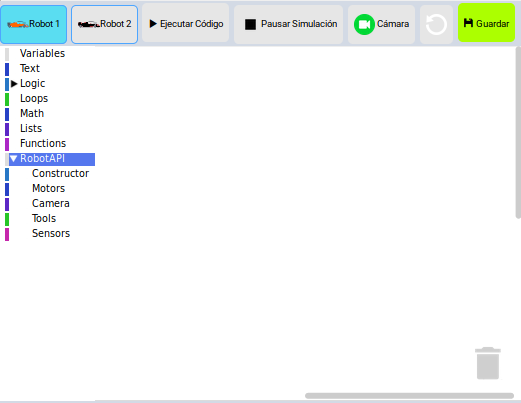
\includegraphics[width=5.5cm, height=4cm]{img/competitivoEditorScratch.png}
                 \label{fig:ir}
                \end{subfigure}
                \begin{subfigure}{\textwidth}
                 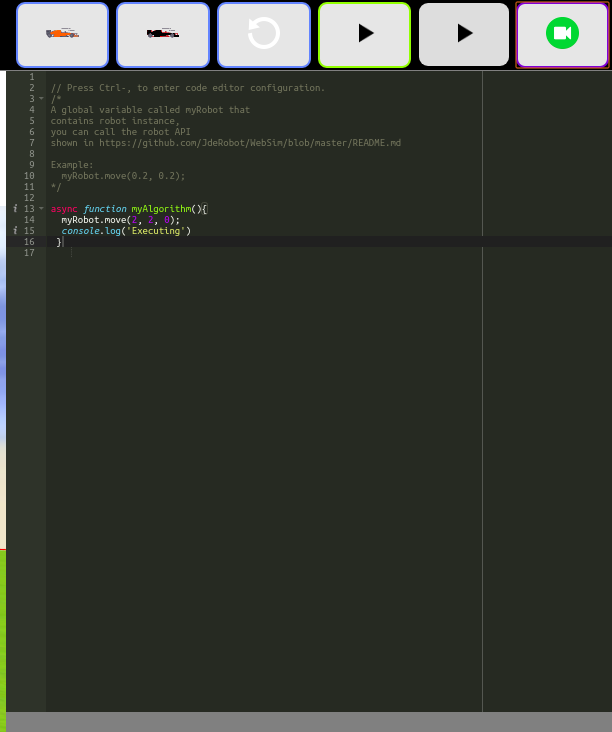
\includegraphics[width=3cm, height=4cm]{img/competitiveEditorJavascript.png}
                \label{fig:vision}
                \end{subfigure}
                \end{figure}
		\end{frame}
		
		\begin{frame}
			\frametitle{\LARGE{Ejercicios competitivos: Atraviesa bosque}}
			
	\begin{minipage}{.48\textwidth}
      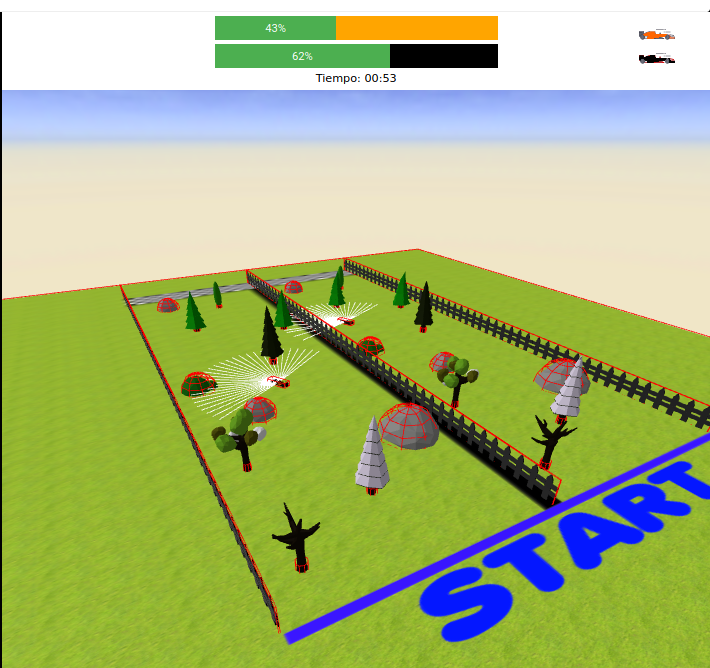
\includegraphics[scale=0.18]{img/evaluador_forest.png}
        \end{minipage}
      \begin{minipage}{.50\textwidth}
      \begin{itemize}
      \begin{itemize}{}\itemsep5pt
          \item \% distancia recorrida
          \item Mismo recorrido 
      \end{itemize}
       \end{itemize}
    \end{minipage}
		\end{frame}
		
		\begin{frame}
			\frametitle{\LARGE{Ejercicios competitivos: Siguelíneas visión}}
			   \begin{minipage}{.50\textwidth}
      \begin{itemize}
          \begin{itemize}{}\itemsep5pt
              \item \% distancia recorrida
              \item Puente primitivas \textit{A-Frame}
          \end{itemize}
       \end{itemize}
    \end{minipage}
		\begin{minipage}{.48\textwidth}	
	         \href{https://youtu.be/OaA7_wsXhk8}{
            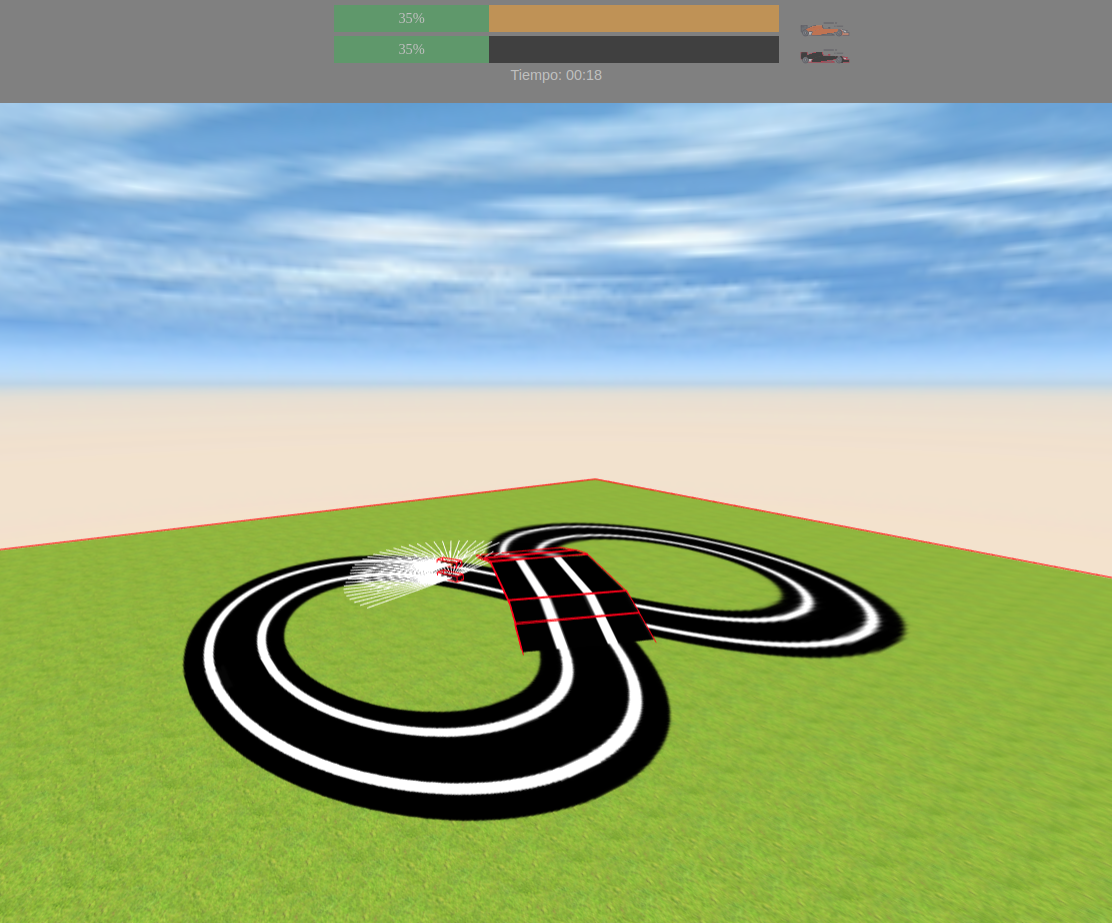
\includegraphics[scale=0.14]{img/evaluator_follow_line.png}}
            \scriptsize{\url{https://youtu.be/OaA7_wsXhk8}} 
        \end{minipage}
		\end{frame}
		

		\begin{frame}
			\frametitle{Ejercicios competitivos: Gato-ratón}

		\begin{minipage}{.48\textwidth}	
	         \href{https://youtu.be/Ez9MSthNWqA}{
            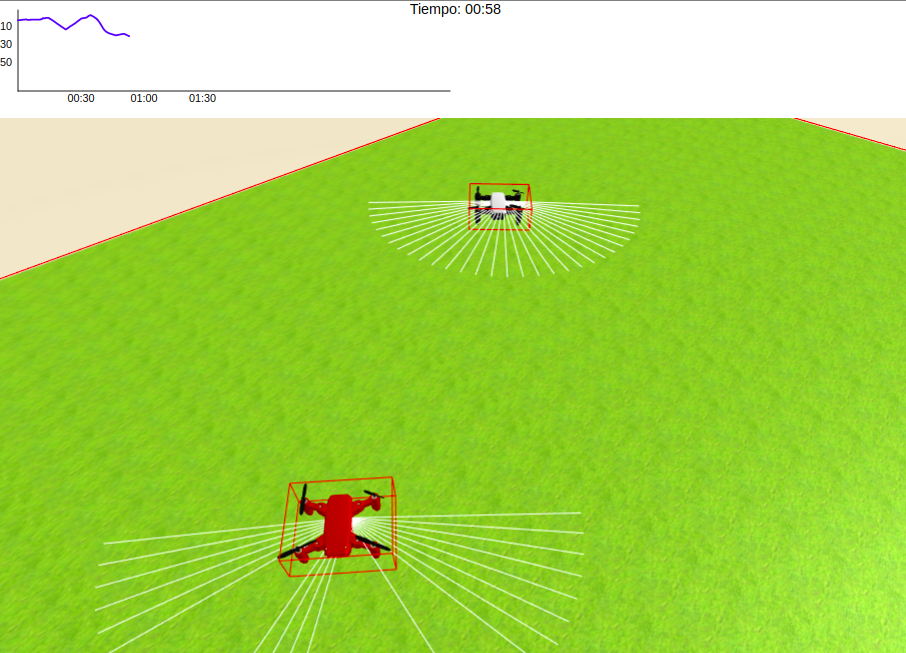
\includegraphics[scale=0.18]{img/evaluador_drone.png}}
            \scriptsize{\url{https://youtu.be/Ez9MSthNWqA}}
        \end{minipage}
        \begin{minipage}{.50\textwidth}
      \begin{itemize}
          \begin{itemize}{}\itemsep5pt
              \item Distancia \textit{drones} en gráfica
              \item Módulo \textit{agents} 
          \end{itemize}
       \end{itemize}
    \end{minipage}
		\end{frame}
		
		\begin{frame}{\Large{Ejercicios competitivos: Gato-ratón evaluador}}
		  \begin{minipage}{.4\textwidth}
      \begin{itemize}
      \begin{itemize}{}\itemsep5pt
          \item Distancia
          \item Gráfica
          \item Cronómetro
          \end{itemize}
      \end{itemize}
    \end{minipage}
		  \begin{minipage}{.58\textwidth}
      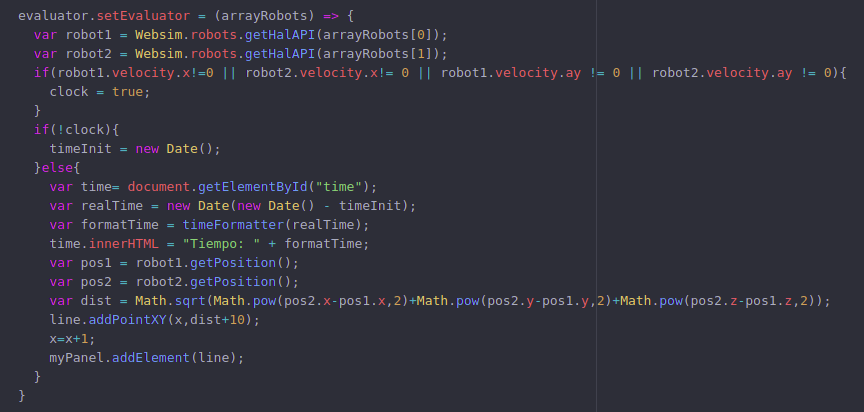
\includegraphics[width=6.75cm, height=4.8cm]{img/drone_evaluator.png}
        \end{minipage}
		\end{frame}

	\section{Conclusiones}
		\begin{frame}
			\frametitle{Conclusiones}
			\begin{itemize}
				\item Soporte a \textit{drones}. \checkmark
				\item Teleoperadores y ficheros de configuración. \checkmark
				\item Ejercicios individuales. \checkmark
				\item Ejercicios competitivos: 
				agentes y evaluadores. \checkmark
			\end{itemize}
		\end{frame}
	
			\begin{frame}
			\frametitle{Líneas futuras}
			\begin{itemize}
				\item \textit{WebWorkers}.
				\item Control en posición interrumpible.
			\end{itemize}
		\end{frame}
	\appendix
	\backupbegin
% 	  \begin{frame}
% 	    \frametitle{Backup slide 1}
% 	  \end{frame}
	\backupend
\end{document}